\subsection{Cohesive laws}
\label{sec:cohesive-laws}

\subsubsection{Linear Irreversible Law\matlabel{ssect:smm:cl:coh-snozzi}}

\begin{figure}[!hbt]
  \centering
  \subfloat[Linear]{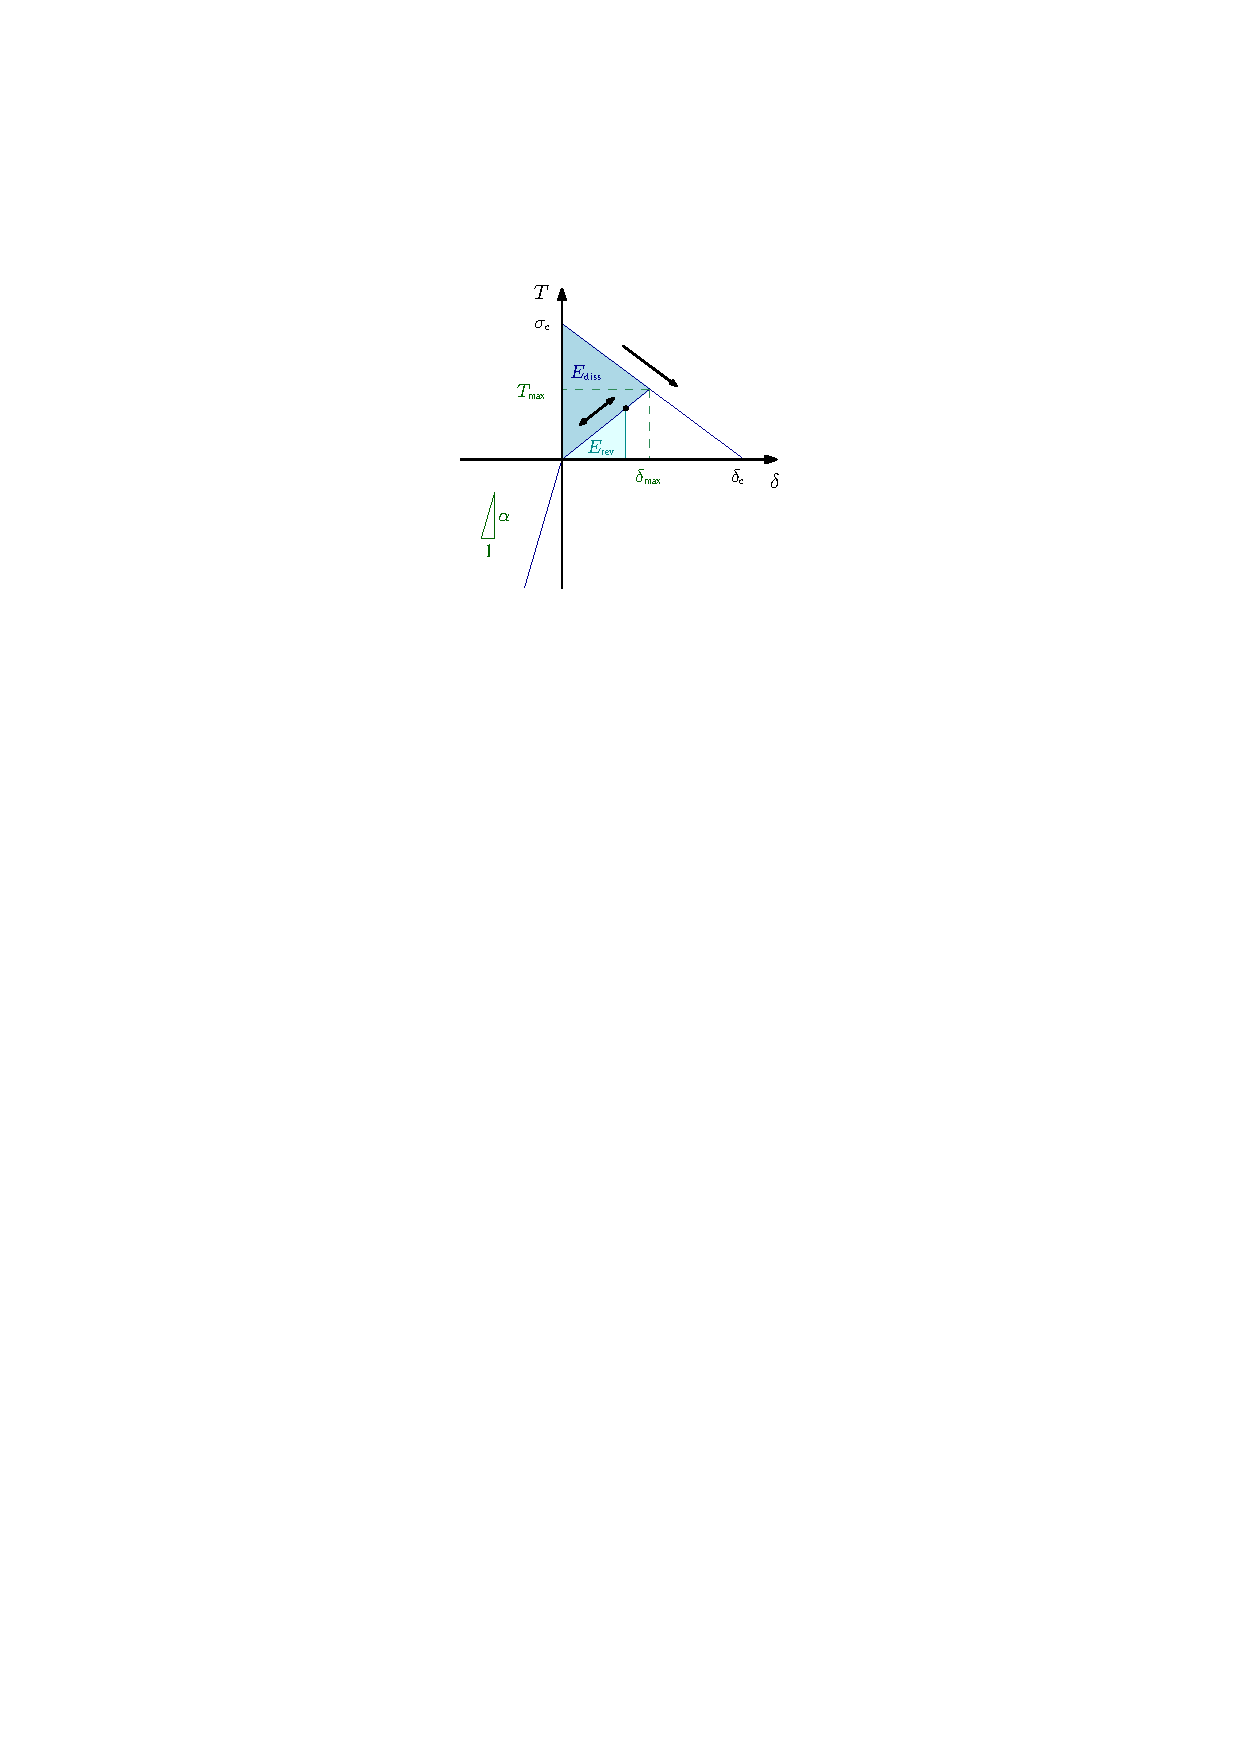
\includegraphics[width=0.4\textwidth]{figures/linear_cohesive_law}}
  \qquad
  \subfloat[Bilinear]{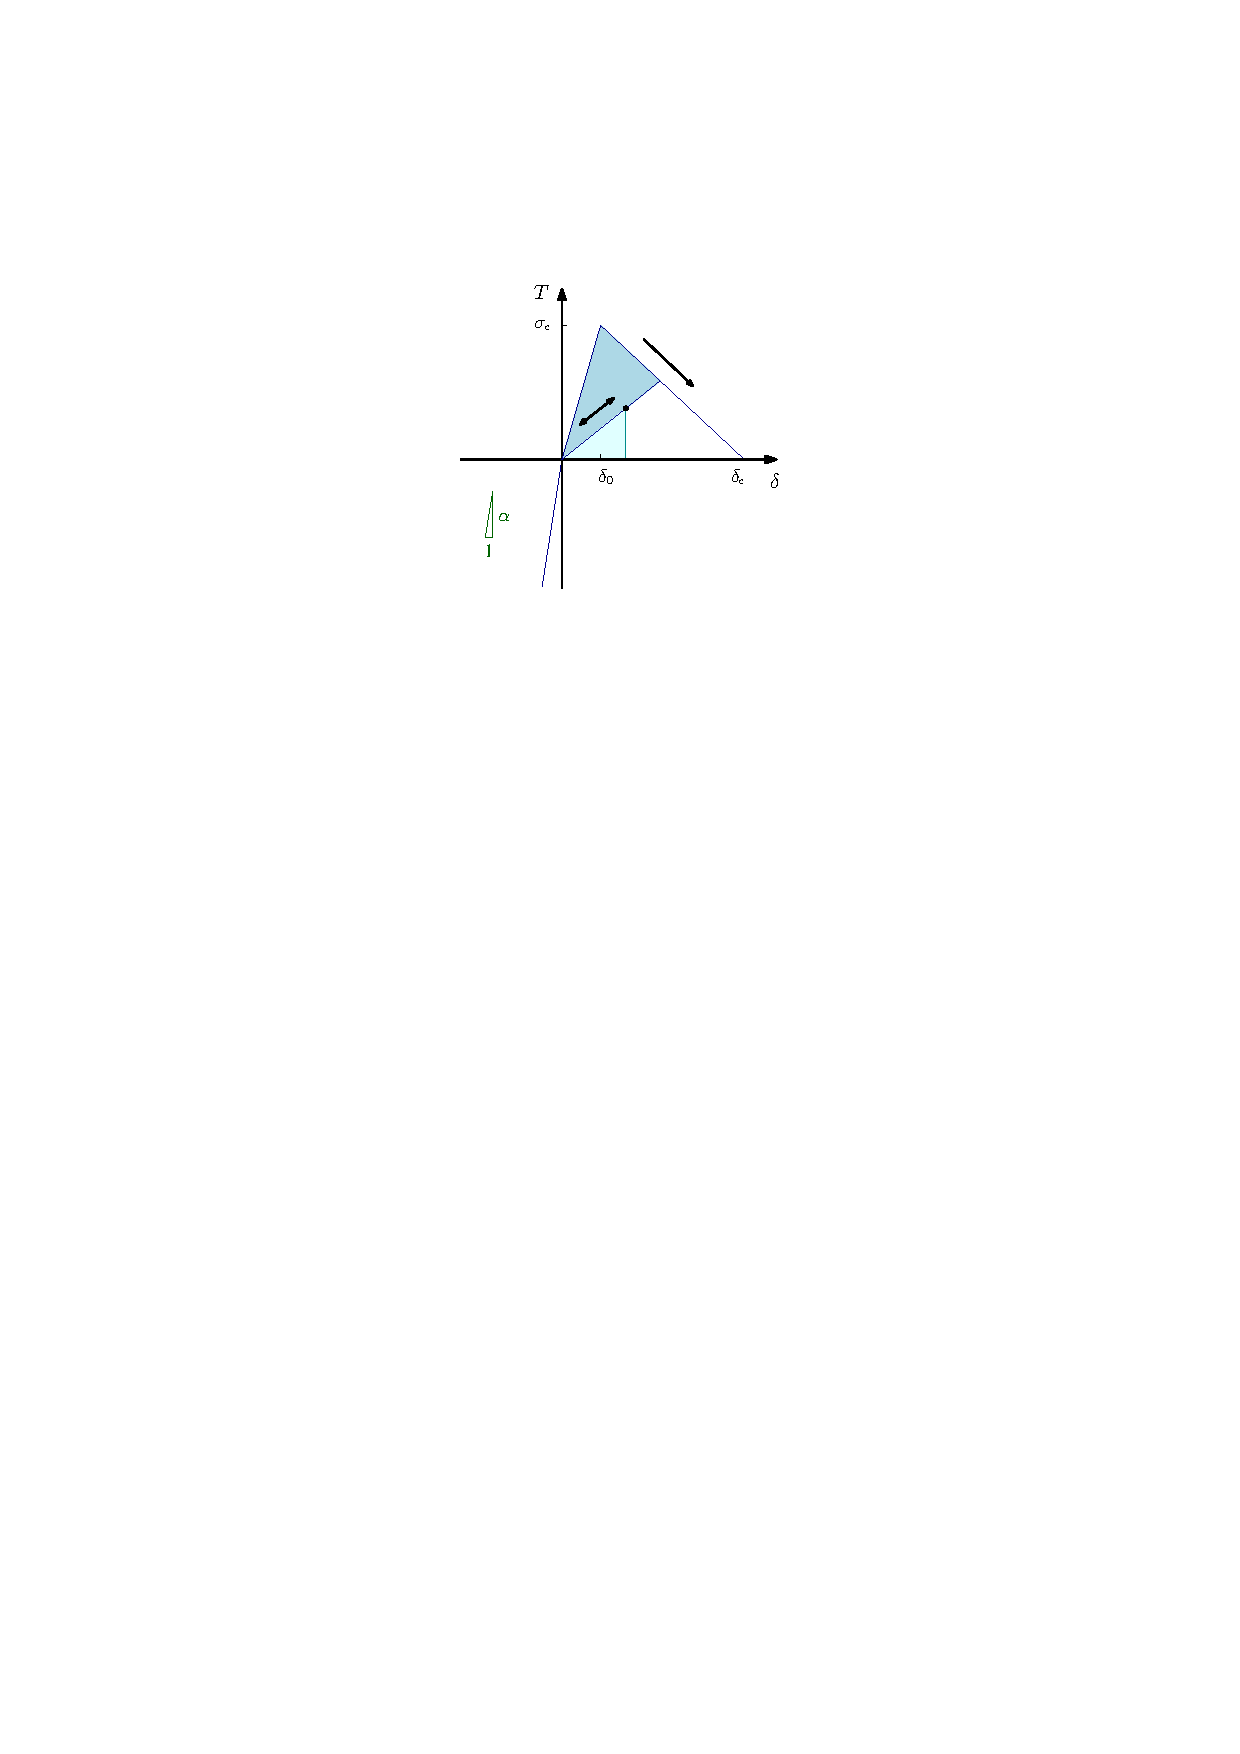
\includegraphics[width=0.4\textwidth]{figures/bilinear_cohesive_law}}
  \caption{Irreversible cohesive laws for explicit simulations.}
  \label{fig:smm:coh:linear_cohesive_law}
\end{figure}

\akantu includes the Snozzi-Molinari~\cite{snozzi_cohesive_2013}
linear irreversible cohesive law (see
Figure~\ref{fig:smm:coh:linear_cohesive_law}). It is an extension to
the Camacho-Ortiz~\cite{camacho_computational_1996} cohesive law in
order to make dissipated fracture energy path-dependent. The concept
of free potential energy is dropped and a new independent parameter
$\kappa$ is introduced:
\begin{equation}
  \kappa = \frac{G_\mathrm{c, II}}{G_\mathrm{c, I}}
\end{equation}

where $G_\mathrm{c, I}$ and $G_\mathrm{c, II}$ are the
necessary works of separation per unit area to open completely a
cohesive zone under mode I and mode II, respectively. Their model yields to the
following equation for cohesive tractions $\vec{T}$ in case of crack
opening ${\delta}$:
\begin{equation}
  \label{eq:smm:coh:tractions}
  \vec{T} = \left( \frac{\beta^2}{\kappa} \Delta_\mathrm{t} \vec{t} +
    \Delta_\mathrm{n} \vec{n} \right)
  \frac{\sigma_\mathrm{c}}{\delta}
  \left( 1- \frac{\delta}{\delta_\mathrm{c}} \right)
  = \hat{\vec T}\,
  \frac{\sigma_\mathrm{c}}{\delta}
  \left( 1- \frac{\delta}{\delta_\mathrm{c}} \right)
\end{equation}

where $\sigma_\mathrm{c}$ is the material strength along the fracture,
$\delta_\mathrm{c}$ the critical effective displacement after which
cohesive tractions are zero (complete decohesion), $\Delta_\mathrm{t}$
and $\Delta_\mathrm{n}$ are the tangential and normal components of
the opening displacement vector $\vec{\Delta}$, respectively. The
parameter $\beta$ is a weight that indicates how big the tangential
opening contribution is. The effective opening displacement is:
\begin{equation}
  \delta = \sqrt{\frac{\beta^2}{\kappa^2} \Delta_\mathrm{t}^2 +
    \Delta_\mathrm{n}^2}
\end{equation}
In case of unloading or reloading $\delta < \delta_\mathrm{max}$,
tractions are calculated as:
\begin{align}
  T_\mathrm{n} &= \Delta_\mathrm{n}\,
  \frac{\sigma_\mathrm{c}}{\delta_\mathrm{max}}
  \left( 1- \frac{\delta_\mathrm{max}}{\delta_\mathrm{c}} \right) \\
  T_\mathrm{t} &= \frac{\beta^2}{\kappa}\, \Delta_\mathrm{t}\,
  \frac{\sigma_\mathrm{c}}{\delta_\mathrm{max}}
  \left( 1- \frac{\delta_\mathrm{max}}{\delta_\mathrm{c}} \right)
\end{align}
so that they vary linearly between the origin and the maximum attained
tractions. As shown in Figure~\ref{fig:smm:coh:linear_cohesive_law},
in this law, the dissipated and reversible energies are:
\begin{align}
  E_\mathrm{diss} &= \frac{1}{2} \sigma_\mathrm{c}\, \delta_\mathrm{max}\\[1ex]
  E_\mathrm{rev} &= \frac{1}{2} T\, \delta
\end{align}
Moreover, a damage parameter $D$ can be defined as:
\begin{equation}
  D = \min \left(
    \frac{\delta_\mathrm{max}}{\delta_\mathrm{c}},1 \right)
\end{equation}
which varies from 0 (undamaged condition) and 1 (fully
damaged condition). This variable can only increase because damage is
an irreversible process. A simple penalty contact model has been incorporated
in the cohesive law so that normal tractions can be returned in
case of compression:
\begin{equation}
  T_\mathrm{n} = \alpha \Delta_\mathrm{n} \quad\text{if
    $\Delta_\mathrm{n} < 0$}
\end{equation}
where $\alpha$ is a stiffness parameter that defaults to zero. The
relative contact energy is equivalent to reversible energy but in
compression.

The material name of the linear decreasing cohesive law  is
\code{material\_cohesive\_linear} and its parameters with their
respective default values are:
\begin{itemize}
\item \code{sigma\_c}: 0
\item \code{delta\_c}: 0
\item \code{beta}: 0
\item \code{G\_c}: 0
\item \code{kappa}: 1
\item \code{penalty}: 0
\end{itemize}
where \code{G\_c} corresponds to $G_\mathrm{c, I}$. A random number
generator can be used to assign a random $\sigma_\mathrm{c}$ to each
facet following a given distribution (see
Section~\ref{sect:smm:CL}). Only one parameter between \code{delta\_c}
and \code{G\_c} has to be specified. For random $\sigma_\mathrm{c}$
distributions, the chosen parameter of these two is kept fixed and the
other one is varied.

The bilinear constitutive law works exactly the same way as the linear
one, except for the additional parameter \code{delta\_0} that by
default is zero. Two examples for the extrinsic and intrinsic cohesive
elements and also an example to assign different properties to
intergranular and transgranular cohesive elements can be found in
the folder \code{\examplesdir/cohesive\_element/}.

\subsubsection{Linear Cohesive Law with Fatigue\matlabel{ssect:smm:cl:coh-fatigue}}

This law represents a variation of the linear irreversible cohesive
law of the previous section, that removes the hypothesis of elastic
unloading-reloading cycles. With this law, some energy is dissipated
also during unloading and reloading with hysteresis. The
implementation follows the work of~\cite{nguyen2001}. During the
unloading-reloading cycle, the traction increment is computed as
\begin{equation}
  \dot{T} =
  \begin{cases}
    K^- \, \dot{\delta} & \text{if $\dot{\delta} < 0$} \\
    K^+ \, \dot{\delta} & \text{if $\dot{\delta} > 0$} \\
  \end{cases}
\end{equation}
where $\dot{\delta}$ and $\dot{T}$ are respectively the effective
opening displacement and the cohesive traction increments with respect
to time, while $K^-$ and $K^+$ are respectively the unloading and
reloading incremental stiffness. The unloading path is linear and
results in an unloading stiffness
\begin{equation}
  K^- = \frac{T_\mathrm{max}}{\delta_\mathrm{max}}
\end{equation}
where $T_\mathrm{max}$ and $\delta_\mathrm{max}$ are the maximum
cohesive traction and the effective opening displacement reached
during the precedent loading phase. The unloading stiffness remains
constant during the unloading phase. On the other hand the reloading
stiffness increment $\dot{K}^+$ is calculated as
\begin{equation}
  \dot{K}^+ =
  \begin{cases}
    - K^+ \, \dot{\delta} / \delta_\mathrm{f} & \text{if $\dot{\delta}
      > 0$} \\
    \left( K^+ - K^- \right) \, \dot{\delta} / \delta_\mathrm{f} &
    \text{if $\dot{\delta} < 0$}
  \end{cases}
\end{equation}
where $\delta_\mathrm{f}$ is a material parameter (refer
to~\cite{vocialta15} for more details). During unloading the stiffness
$K^+$ tends to $K^-$, while during reloading $K^+$ gets decreased at
every time step. If the cohesive traction during reloading exceeds the
upper limit given by equation~\eqref{eq:smm:coh:tractions}, it is
recomputed following the behavior of the linear decreasing cohesive
law for crack opening.

\subsubsection{Exponential Cohesive Law\matlabel{ssect:smm:cl:coh-exponential}}

Ortiz and Pandolfi proposed this cohesive law in 1999~\cite{ortiz1999}.  The
traction-opening equation for this law is as follows:
\begin{equation}
  \label{eq:exponential_law}
  T = e \sigma_c \frac{\delta}{\delta_c}e^{-\delta/ \delta_c}
\end{equation}
This equation is plotted in Figure~\ref{fig:smm:CL:ECL}. The term
$\partial{\vec{T}}/ \partial{\delta}$ of
equation~\eqref{eq:cohesive_stiffness} after the necessary derivation
can expressed as
\begin{equation}
  \label{eq:tangent_cohesive}
  \frac{\partial{\vec{T}}} {\partial{\delta}} = \hat{\vec{T}} \otimes
  \frac                       {\partial{(T/\delta)}}{\partial{\delta}}
  \frac{\hat{\vec{T}}}{\delta}+ \frac{T}{\delta}  \left[ \beta^2 \mat{I} +
  \left(1-\beta^2\right) \left(\vec{n} \otimes \vec{n}\right)\right]
\end{equation}
where
\begin{equation}
  \frac{\partial{(T/ \delta)}}{\partial{\delta}} = \left\{\begin{array} {l l}
      -e  \frac{\sigma_c}{\delta_c^2  }e^{-\delta  /  \delta_c} &  \quad  if
      \delta \geq \delta_{max}\\
      0 & \quad if \delta < \delta_{max}, \delta_n > 0
    \end{array} \right.
\end{equation}

As regards the behavior in compression, two options are available:
a contact penalty approach with stiffness following the formulation of
the exponential law and a contact penalty approach with constant
stiffness. In the second case, the stiffness is defined as a function
of the tangent of the exponential law at the origin.

\begin{figure}[!htb]
  \begin{center}
    \includegraphics[width=0.6\textwidth,keepaspectratio=true]{figures/cohesive_exponential.pdf}
    \caption{Exponential cohesive law}
    \label{fig:smm:CL:ECL}
  \end{center}
\end{figure}


%%% Local Variables:
%%% mode: latex
%%% TeX-master: "manual"
%%% End:
